%!TEX root = ../Dokumentation.tex

\chapter{Konzeption}

\section{Die Idee}

Zu Beginn des Projektes ging es um das Finden eines geeigneten Anwendungsfalls aus der Realität. Für diesen sollte das geforderte System, eine sinnvolle Ergänzung für mögliche Anwender darstellen.\\
Zum einen muss die Möglichkeit bestehen, Informationen direkt auszutauschen und zum anderen sollte eine Art Benachrichtigungssystem existieren, bei denen die Interessenten nur beim Eintreten bestimmter Ereignisse informiert werden müssen.\\
Nach Überlegung fiel dabei die Wahl auf das Thema Film und Fernsehen und wurde im Spezielleren auf Serien eingegrenzt. Sinnvoll erscheint eine Umsetzung dieses Thema aufgrund der regelmäßigen Ausstrahlung von Folgen einer bestimmten Serie.\\
Während man für einen Film lediglich einmal die Ausstrahlungszeit in Erfahrung bringen muss, würde sich dieser Schritt bei Serieninteressierten Woche für Woche wiederholen. Dazu kommen kurzfristige Änderung im Fernsehkalender, die im unpassenden Fall dazu führen, dass eventuell Folgen verpasst werden. Schaut jemand nicht nur eine Serie, sondern hat eine Art festen Wochenplan, so kann hierbei auch der Überblick darüber verloren gehen, welche Folge man eigentlich zuletzt gesehen hat oder wie die Serie hieß, die einem neuliche empfohlen wurde.

\vspace{0.2cm}

Mit dieser grundlegenden Überlegung ging es an das Konzipieren des Funktionsumfangs des Systems unter dem Projekttitel \textbf{Serientracker}.\\
Die Idee ist, dass Serieninteressierte\footnote[1]{Innerhalb des Kontext wird für den Benutzertyp des Anwenders/Nutzers auch diese Bezeichnung verwendet werden, da diese Personengruppe in ihrer Funktion die Benutzer des Systems darstellen werden.} die Möglichkeit besitzen bestimmte Serien zu favorisieren und Meldungen zu gewissen Themen abonnieren können. Er soll Zugriff auf einen Pool von Serien bekommen, die auf einem Server gespeichert und verwaltet werden. Der Benutzer erhält dann zu seinen Lieblingsserien Benachrichtigungen, sobald eine Episode dieser Serie im TV ausgestrahlt wird. Wenn vorher noch das Genre Comedy abonniert wurde, so erhält er zudem noch eine Benachrichtigung, welche Serien dieses Typs aktuell so laufen.\\
Außerdem soll die Möglichkeit bestehen eine Episode zu bewerten und als gesehen/ungesehen zu markieren. Diese Verwaltung findet innherhalb von privat angelegten Listen statt, die neben der klassischen Seen/Unseen Form auch als Watchlist oder ähnliches definiert werden kann.

\vspace{0.2cm}

Die \textbf{Server-Anwendung} soll die Nutzer über die TV-Austrahlung einer Episode zu einem Zeitraum informieren, die sich der Benutzer selbst definiert hat. Er kann demnach entscheiden, ob ihm eine Benachrichtigung für die ganze Woche genügt, ob er jeden Morgen über den aktuellen Tag informiert werden möchte oder eine Meldung 5 Minuten vor Sendestart ausreicht, da er planmäßig zu Hause sein wird.

\vspace{0.2cm}

Ein \textbf{Content-Admin} soll erweiterte Rechte bekommen, um die Content-Verwaltung zu übernehmen. Die Anwendung soll das Anlegen, Bearbeiten und Löschen von Serien bzw Episoden ermöglichen. Zudem ist somit das Korrigieren von Fehlern möglich, die von Usern eingeschickt werden oder die aufgrund von Planänderungen anfallen.

\vspace{0.2cm}

Als möglicher Zusatz ist eine Einbindung von Freunden geplant. Nutzer sollen sich gegenseitig hinzufügen/abonnieren können um sich gegenseitig zu benachrichtigen. Zum Beispiel in Form von \textit{Freund X schaut gerade Y}, \textit{Freund Z hat Serie/Episode mit 8,0 bewertet} oder \textit{Freund Y empfiehlt dir Serie W}. Ob dieser Ansatz innerhalb des Projektes realisiert wird, hängt vom vorranschreiten der Umsetzung  und der damit einhergehenden Abwägung für das eigentlich Ziel des Projektes ab.

\section{Informationsaustausch}

Zuvor genannte Funktionen würden, für einen Informationsaustausch zwischen Server und Anwendung, hinsichtlich folgender Einstufung der Datenübertragung umgesetzt werden.

\subsection{Synchrone Datenübertragung}

Zum einen hat der Anwender direkt die Möglichkeit auf Informationen in Form von Daten zuzugreifen und diese zu Manipulieren.

\begin{itemize}
\item
Serien-Interessierte
  \begin{itemize}
  \item
    Markieren von Episoden
      \begin{itemize}
      \item
      Gesehen/Nicht gesehen
      \end{itemize}
    \item
    Bewertung einer Episode
        \begin{itemize}
        \item
        Kommentar
        \item
        Bewertung in Zahlen
        \end{itemize}
     \item
     Fehlermeldung
      \begin{itemize}
      \item
        geänderte Sendezeit, fehlerhaftes Datum
        \end{itemize}
     \item
     Listen
      \begin{itemize}
      \item
      Ausgabe (Un)Watched
      \item
      Ausgabe vorhandene Serien
      \item
      Ausgabe Follower/Following
      \end{itemize}
     \item
     Favorisierung
        \begin{itemize}
        \item
        Anlegen
        \item
        Löschen
        \item
        Bearbeiten
          \begin{itemize}
          \item
            Zeitpunkt der Benachrichtigung
            \end{itemize}
    \end{itemize}
  \end{itemize}
  \item
  Content-Admin
    \begin{itemize}
    \item
    Verwaltung der Episoden
      \begin{itemize}
      \item
      Anlegen
      \item
      Löschen
      \item
      Bearbeiten
      \end{itemize}
    \end{itemize}
\end{itemize}


\subsection{Asynchrone Datenübertragung}

Ein weiterer Aspekt ist das Anfordern von Informationen, wobei die entsprechenden Informationen von Seiten des Servers von Bedingungen abhängig gesendet werden, was auch mehrfach geschehen kann.

\begin{itemize}
\item
Serien-Interessierte
  \begin{itemize}
  \item
    Benachrichtung bei TV-Austrahlung
    \item
    Freunde mit gleicher Favorisierung bei Serienstart mit Check-in benachrichtigen
      \begin{itemize}
      \item
         Freund X schaut auch W
         \end{itemize}
    Empfehlung einer Serie von Freund(e) anzeigen
    \end{itemize}
\item
Content-Admin
  \begin{itemize}
  \item
    Benachrichtung bei Fehlermeldung durch User
    \end{itemize}
\end{itemize}

\subsection{Kommunikationsabläufe}
Im Rahmen des Konzeptes wurden zwischen dem Server und dem User (hier repräsentativ für die Anforderung seitens der Anwendung) folgende Kommunikationsabläufe identifiziert.\\
Die synchronen Interaktionen werden vom User iniziiert und greifen auf die beim Server abgelegten Datensätze zu. Dabei hat jeder User die Möglichkeit eine einfache Anzeige der Daten anzufordern oder eine Serie den Favoriten hinzuzufügen. Usern mit erweiterten Adminrechten wird hierbei auch die Manipulation der Daten gewährleistet, um eine Verwaltung zu ermöglichen. Die entsprechende Repräsentation der Information wird vom Server wieder an den User zurückgegeben.\\
Diese Ansätze werden über einen RESTful Webservice umgesetzt und mit entsprechenden GET, POST, PUT und DELETE Methoden realisiert.

\begin{figure}[H]
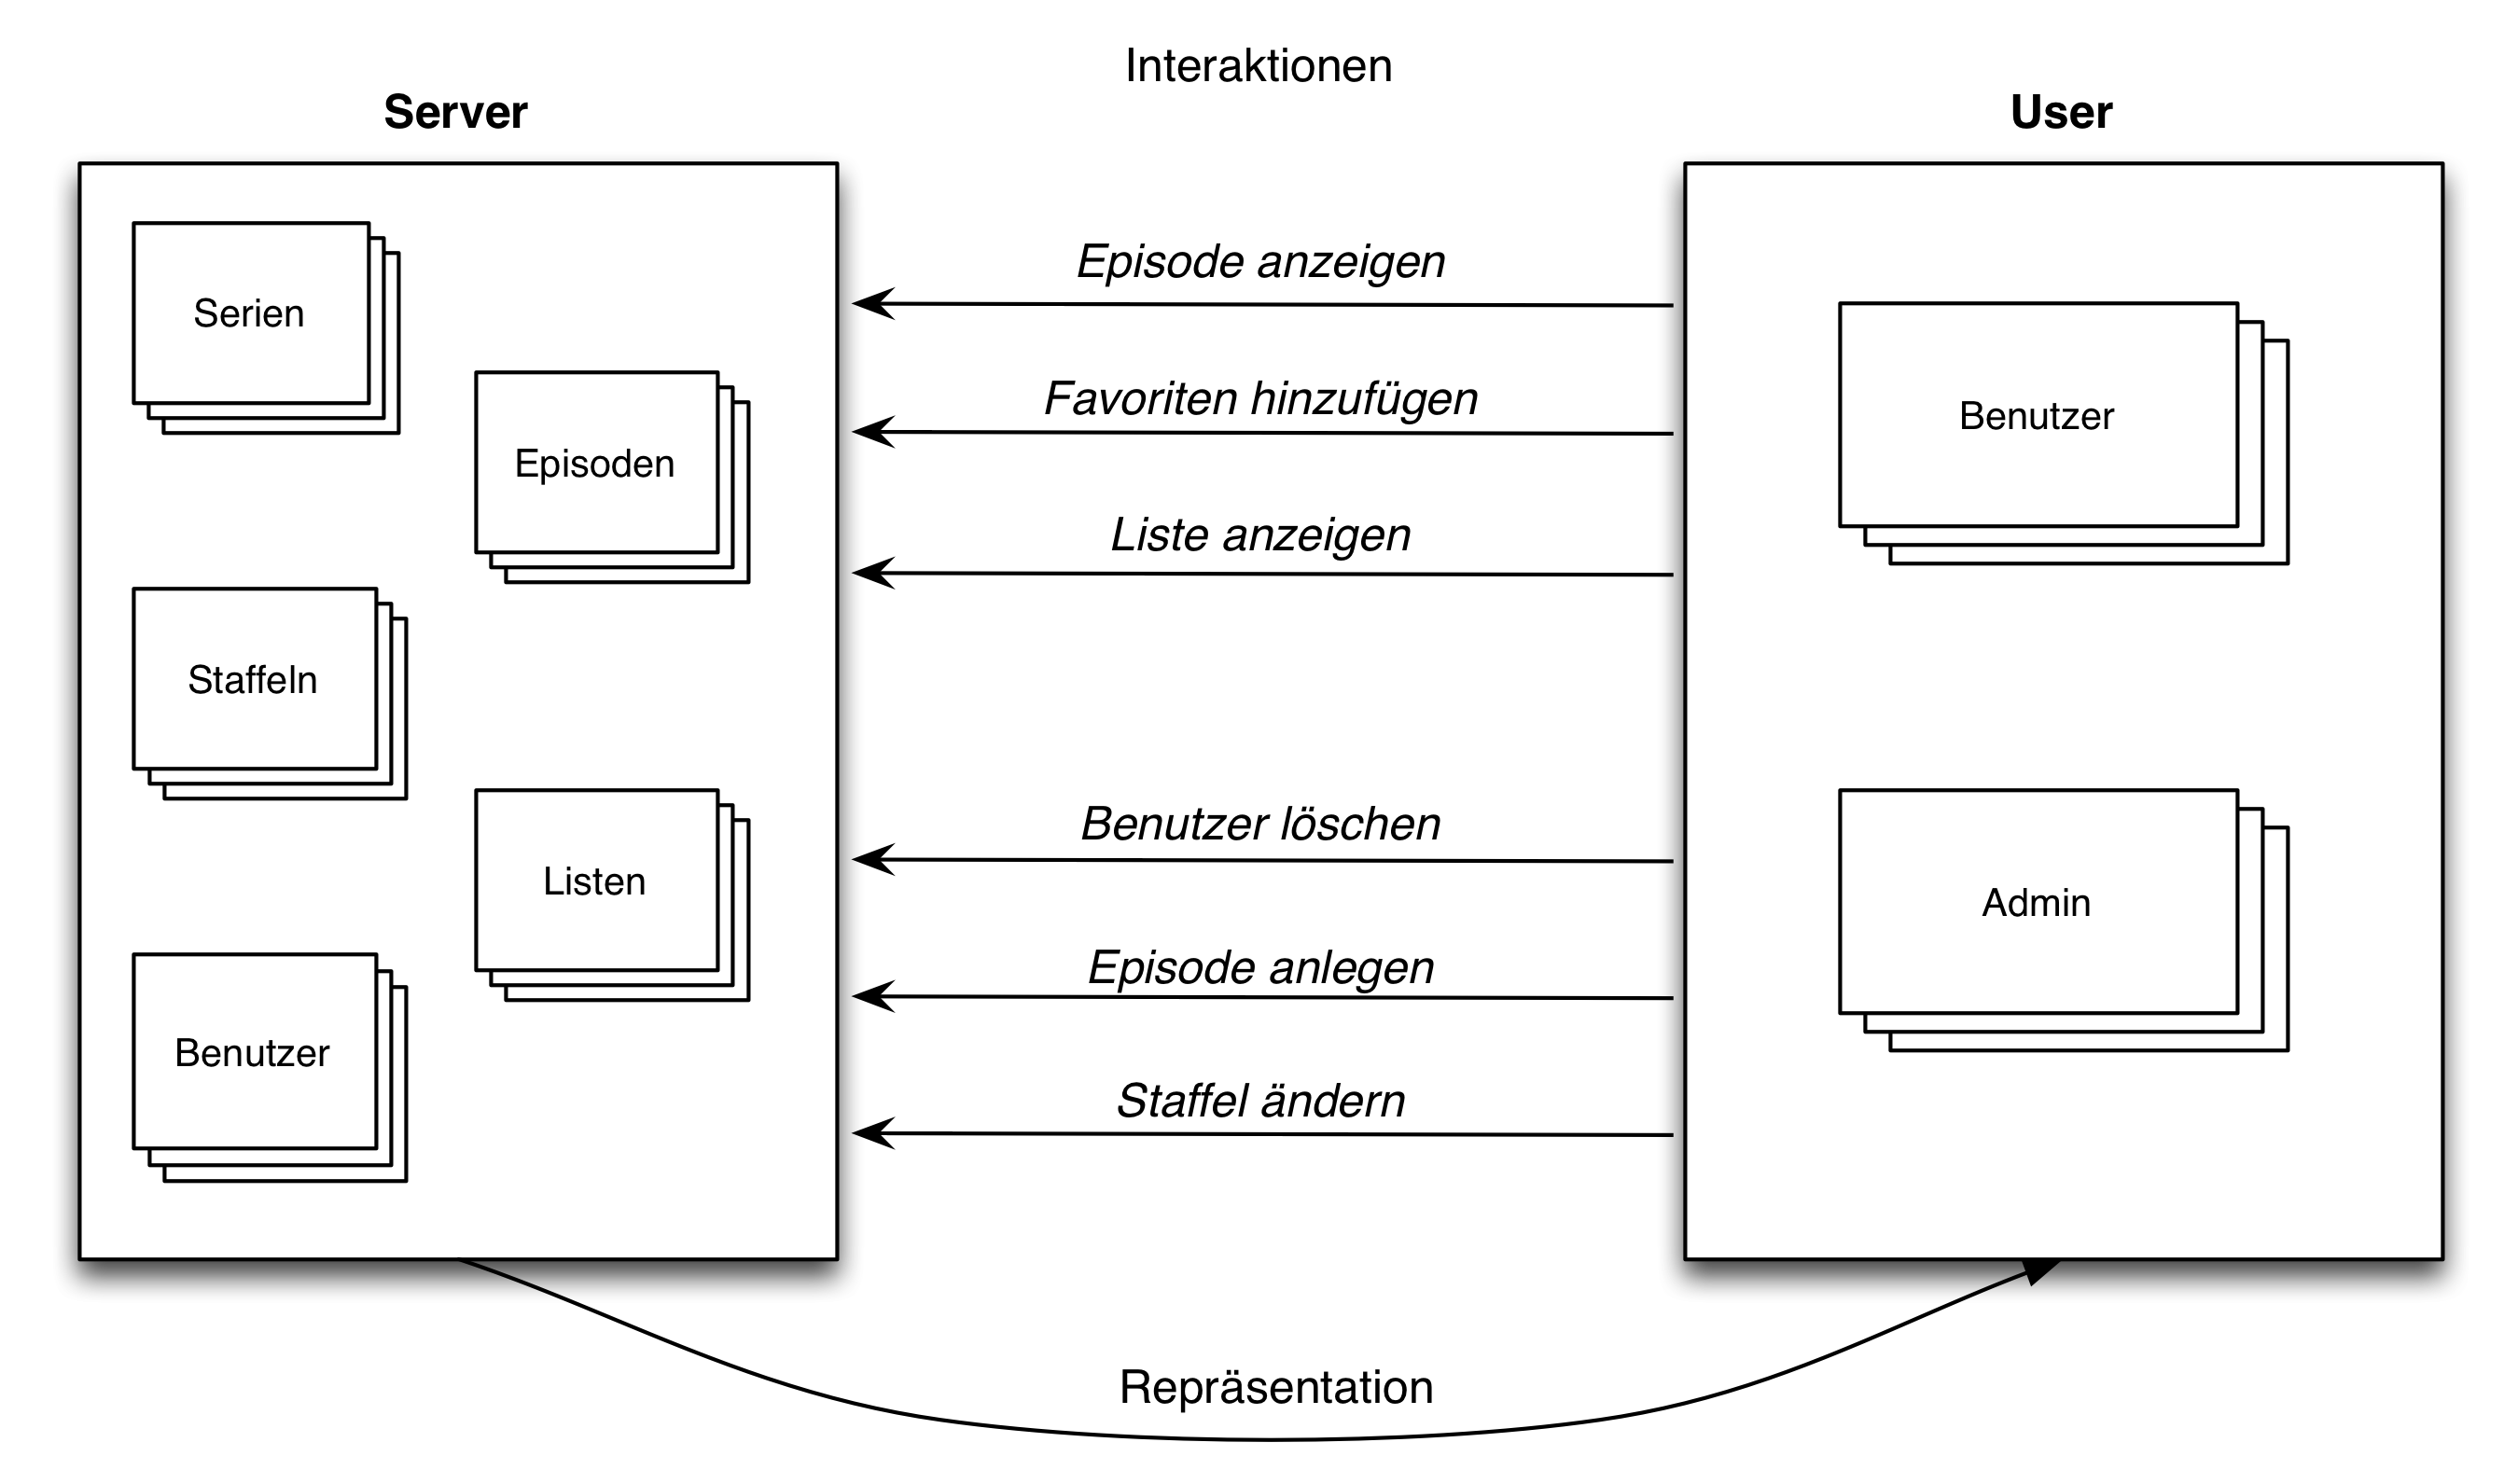
\includegraphics[width=1\textwidth]{../images/kommunikationsablaeufe.png}
\caption{Synchrone Kommunikationsabläufe}
\label{kommunikationsablaeufe}
\end{figure}

Die Asynchronen Kommunikationsabläufe liefern Informationen bei bestimmten Events vom Server an die entsprechenden User als Empfänger. Dieser Ansatz wird mit Hilfe von XMPP realisiert werden und ist im Kapitel 3.4 genauer dargelegt.

\begin{figure}[H]
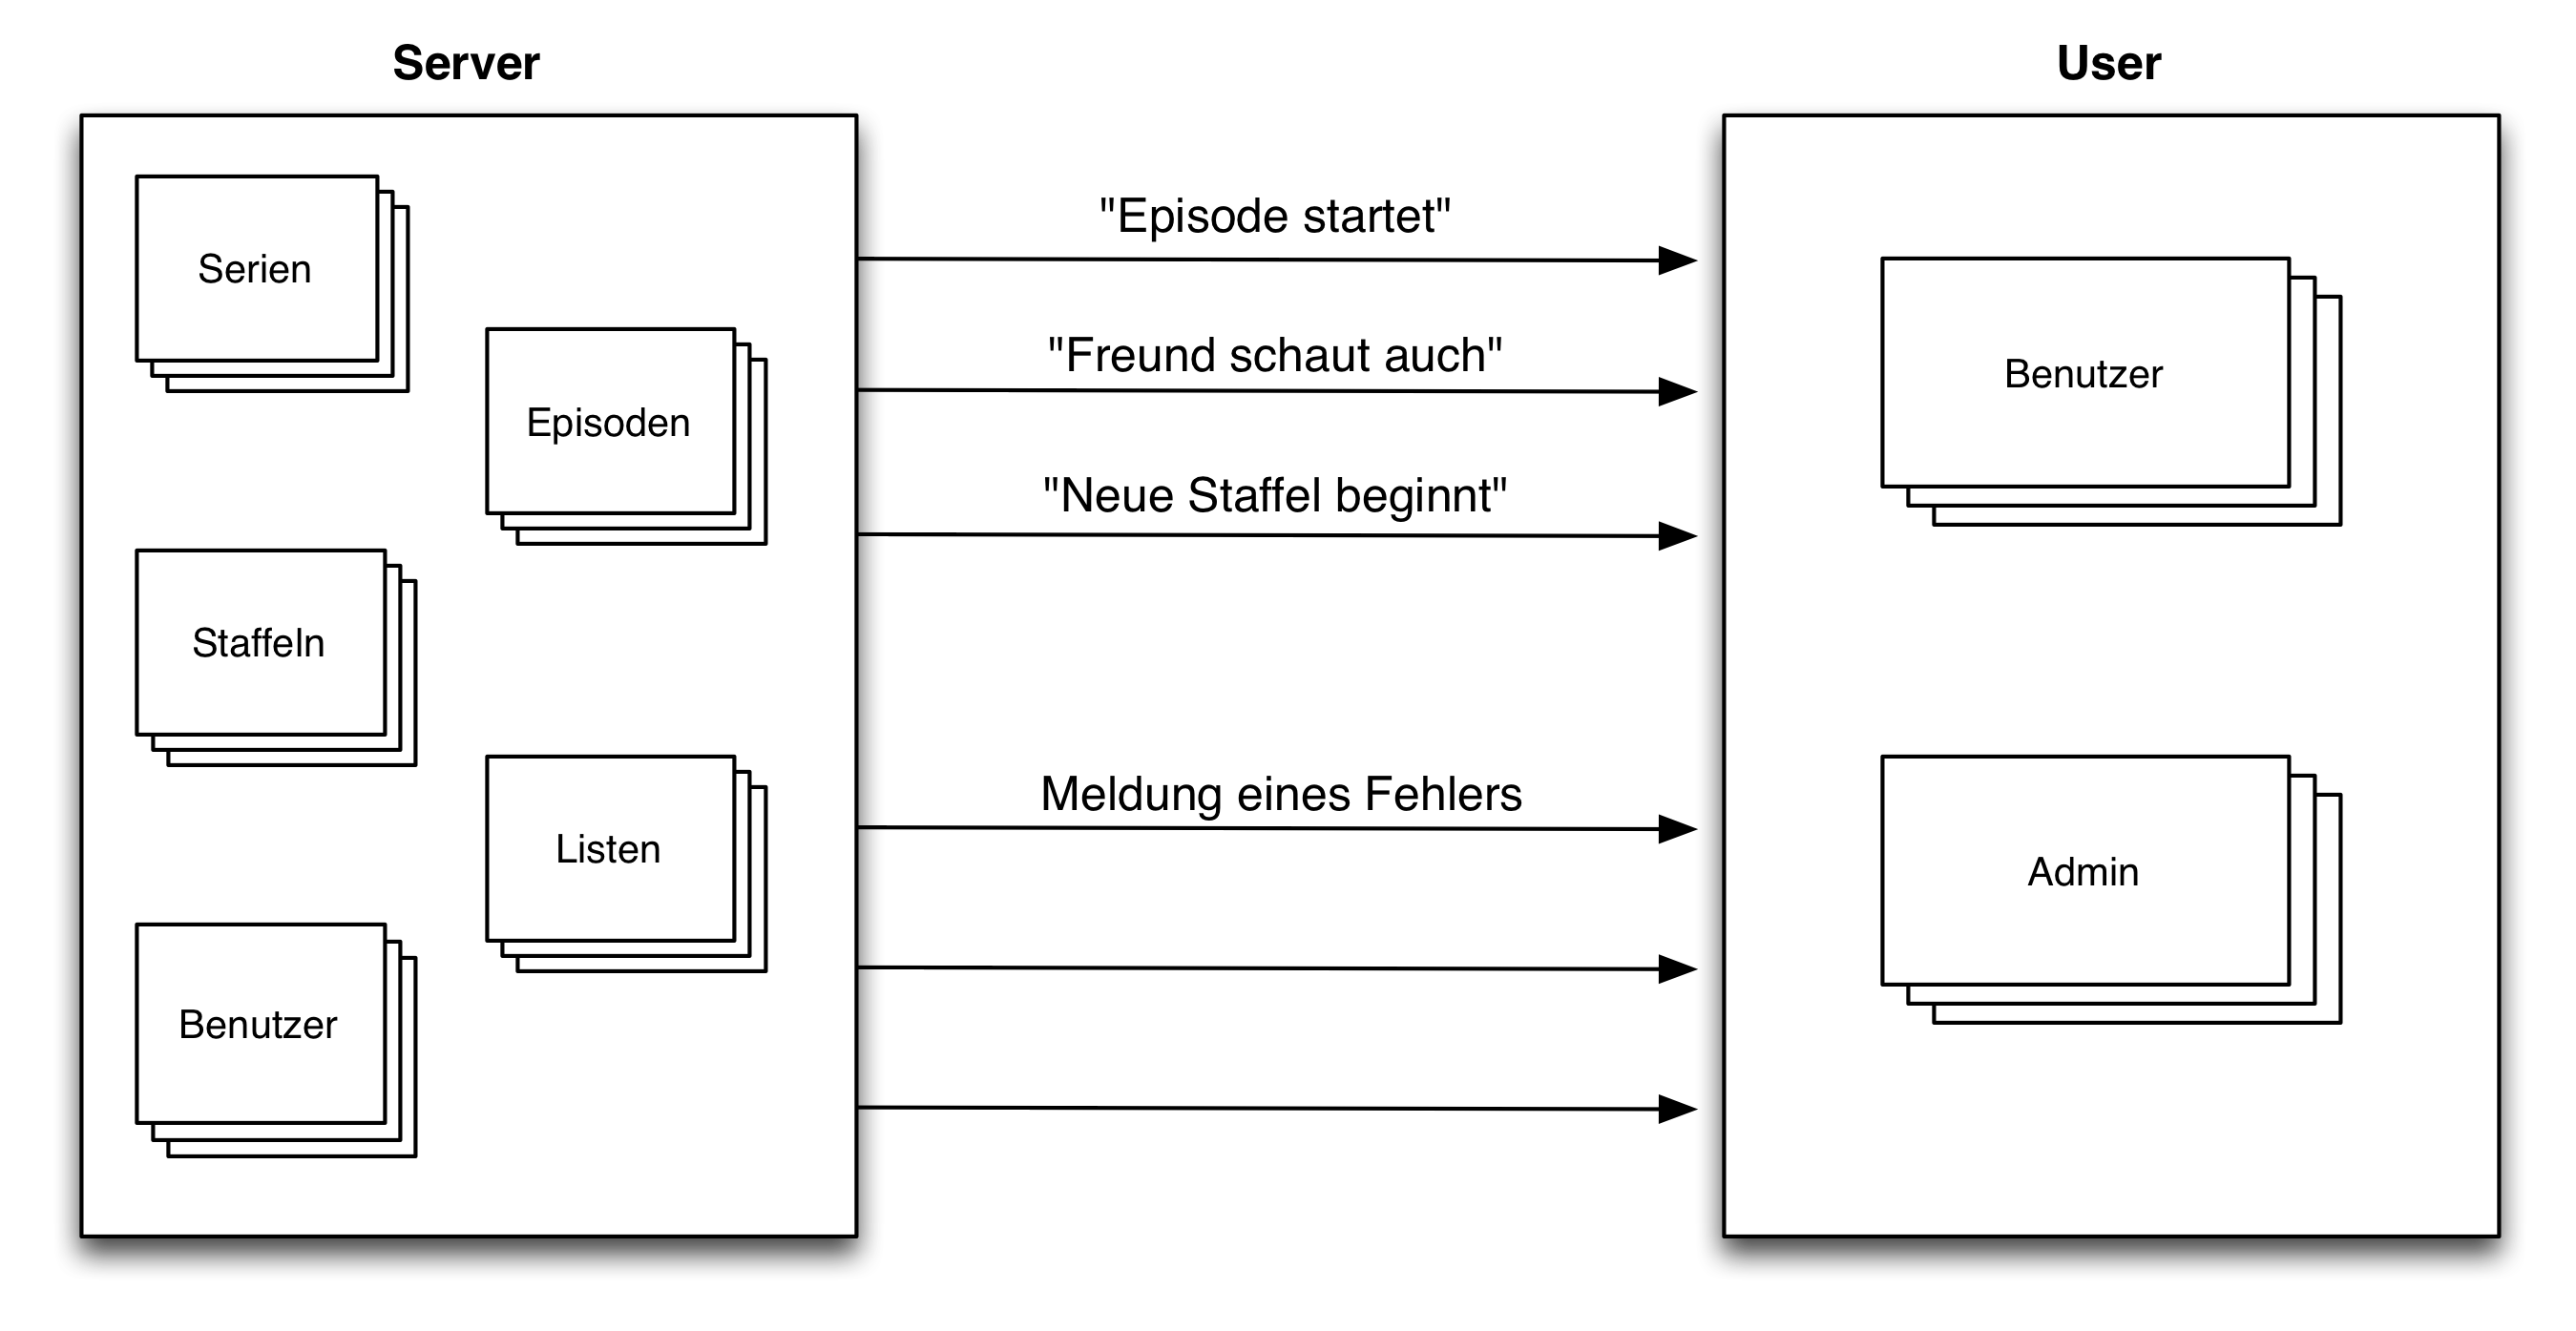
\includegraphics[width=1\textwidth]{../images/kommunikationsablaeufeAsynchron.png}
\caption{Asynchrone Kommunikationsabläufe}
\label{kommunikationsablaeufeAsynchron}
\end{figure}
